\section{Aufgabe 1: Entscheidungsbäume}
\subsection{Feature Engineering}

\subsubsection{Analyse der Zielvariable}
Wie Abbildung \ref{fig:disc_target_variable} entnommen werden kann, ist die Ausprägung der Zielvariable ungleich auf beide Klassen verteilt. Die Klassifizierungsgenauigkeit eines Modells muss demnach unter Berücksichtigung der sogenannten \emph{Null Accuracy} bewertet werden. Unter \emph{Null Accuracy} versteht man die Genauigkeit eines Modells, dass unabhängig von allen Eingaben immer die am häufigsten auftretende Klasse vorhersagt. In unserem Fall würde ein Modell, welches immer Regen vorhersagt, eine Klassifizierungsgenauigkeit von 79,39\% erreichen. Das Ziel der nachfolgenden Schritte ist also ein Modell mit einer besseren Klassifizierungsgenauigkeit als die \emph{Null Accuracy} aufzubauen.


\begin{figure}[ht]
	\centering
	\vspace*{-0.9 cm}
	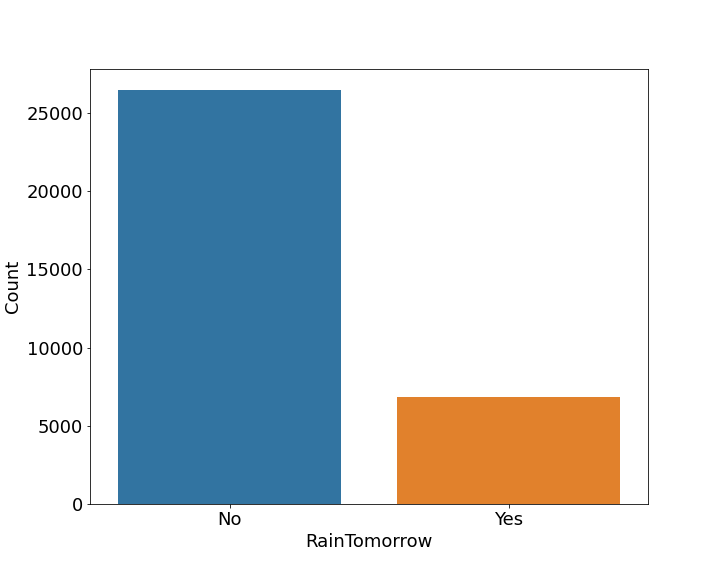
\includegraphics[width = 0.45\textwidth]{Bilder/distribution_target_variable.png}
	\caption{Verteilung der Zielvariable}
	\label{fig:disc_target_variable}
\end{figure}

\subsubsection{Fehlende Werte}
Der zu untersuchende Datensatz beinhaltet fehlende Werte. Im Folgenden werden Methoden beschrieben, wie mit den fehlenden Werte umgegangen wurde:
\begin{description}
	\item[Fehlende Zielvariable:]
	 Im ersten Schritt wurden alle Beobachtungen, welche keinen Wert für die Zielvariable \emph{RainTomorrow} aufweisen, aus dem Datensatz entfernt. Damit wurde die Anzahl an Beobachtungen um 834 auf 33402 reduziert.
	 \item[Spalten mit fehlenden Werten:]
	 In einem nächsten Schritt werden die Spalten aus dem Datensatz entfernt, in denen mehr als 40\% der beinhaltenden Variablen fehlen. Namentlich wurden somit die Spalten \emph{Evaporation, Sunshine, Cloud9am} sowie \emph{Cloud3pm} aus dem Datensatz entfernt. Der Schwellwert von 40\% wurde empirisch festgelegt und hat zu den besten Klassifizierungsergebnissen geführt.
	 \item[Beobachtungen mit fehlenden Werten]
	 Des Weiteren werden Beobachtungen aus dem Datensatz entfernt, von denen mehr als 50\% der Variablen fehlen. Durch diesem Schritt wurden 55 Beobachtungen aus dem Datensatz entfernt.
	 \item[Imputation]
	 Durch die zuvor beschriebenen Methoden ist der Datensatz immer noch  nicht frei von fehlenden Werten. Um diese zu ersetzen, werden für kategorische und numerische Variablen verschiedene Strategien zur Imputation verfolgt. Fehlende numerische Werte werden mit dem Median der jeweiligen Variable ersetzt. Der Median wurde gewählt, da dieser im Vergleich zum Mittelwert robuster gegenüber Ausreißern ist. Für kategorielle Variablen hingegen wird der am häufigsten vorkommende Wert verwendet. Wichtig bei der Ermittlung des Medians bzw. des häufigsten Wertes ist, dass dieser ausschließlich mit Hilfe der Trainingsdaten (siehe Abschnitt \ref{section:train_test_split}) ermittelt wird. Es muss davon ausgegangen werden, dass die Testdaten nicht bekannt sind. Die Ermittlung auf Basis des gesamten Datensatzes, inklusive der Testdaten, würde zu \emph{Data Leakage} führen und ist zu vermeiden. Die auf Basis der Trainingsdaten ermittelten Werte für die Imputation werden auf die Trainings- und Testdaten angewendet.
\end{description}

\subsubsection{Merkmalserstellung und Aufteilung}
Eine weit verbreitete Technik des Feature Engineerings ist die Erstellung zusätzlicher Merkmalen. Somit wurde die Variable \emph{MinMaxDiff} erstellt, welche die Differenz zwischen der minimalen und der maximalen Tages-Temperatur angibt. Des Weiteren wurden die Variablen \emph{PressureDiff, HumidityDiff und WindSpeedDiff} als Differenz der Beobachtungen am Morgen und Abend erstellt. Das Feld \emph{Datum} wurde in die Merkmale \emph{Year, Month} und \emph{Day} aufgeteilt.

\subsubsection{Diskretisierung}
%TODO: Entscheidungsbäume sind doch auch sensibel gegenüber vieler verschiedener Werte... Das wäre noch ein gutes Argument
Die Diskretisierung eines Merkmals kann eine Überanpassung bei der Erstellung von Modellen verhindern, indem der Wertebereich des Merkmals minimiert und somit generalisiert wird. Hierbei muss beachtet werden, dass der Informationsverlust durch die Diskretisierung nicht zu groß ist. Eine Diskretisierung wurde für das Merkmal \emph{Month} durchgeführt, indem es in das Merkmal \emph{Season} umgewandelt wurde. Das Merkmal \emph{Season} fasst immer 3 Monate zu einer Jahreszeit zusammen.

\subsubsection{Kodierung kategorischer Werte}
Um kategorische Werte für weitere Analysen verwenden zu können, müssen diese in numerische Werte umkodiert werden. Hierbei wurden die folgenden Strategien Angewendet:
\begin{description}
	\item[Binäre Kodierung]
	Die Zielvariable \emph{RainTomorrow}, sowie die Variable \emph{RainToday} liegen in den Ausprägungen \emph{Yes} und \emph{No} vor. Für eine weitere Verarbeitung wurden die Ausprägungen in eine numerische binäre Darstellung umgewandelt.
	\item[One-Hot-Kodierung]
	%TODO: One-Hot beschreiben?
	Das neu diskretisierte Merkmal \emph{Season} wird mittels \emph{One-Hot-Kodierung} umgewandelt. Eine \emph{Label-Kodierung}, also eine einfache Kodierung mit einem zufälligen Zahlenwert pro auftretender Variablenausprägung, hat den Nachteil, dass dadurch eine Variable entsteht, die gegebenenfalls metrisch interpretiert wird.
	\item[Ziel-Kodierung]
	Mit Hilfe der Ziel-Kodierung werden die Merkmale \emph{Location, WindGustDir, WindDir9am} und \emph{WindDir3pm} umgewandelt. Hierbei werden die Merkmalsausprägungen als ihren Einfluss auf die Zielvariable kodiert.
\end{description}

\subsubsection{Bereinigung von Ausreißern}
%TODO: Haben wirklich nur die Vairablen ausreißer?? Ich hatte nur die im code untersucht...
Ausreißer können die Performance eines Modells mindern, indem sie als Hebelwerte agieren und somit die Schätzungen der Zielvariable verzerren. Aus diesem Grund werden die Merkmale des Datensatz hinsichtlich ihrer Ausreißer begutachtet. Es wird ersichtlich, dass Merkmale wie \emph{Rainfall} und \emph{WindGustSpeed} abweichende Werte aufweisen. Das Entfernen dieser Werte aus dem Datensatz führt jedoch zu einer schlechteren Performance der im folgenden Abschnitt besprochenen Entscheidungsbäume. Deshalb werden die Beobachtungen nicht aus dem Datensatz entfernt.

\subsubsection{Normalisierung der Daten}
Für Entscheidungsbäume ist eine Normalisierung der Daten nicht Notwendig. Um das \emph{Feature Engineering} jedoch unabhängig vom gewählten Klassifizierer und auch im Hinblick auf neuronale Netze oder \emph{Support Vector Machines} (SVMs) durchzuführen, wird es an dieser Stelle durchgeführt. Die Werte der einzelnen Variablen werden dabei auf den Wertebereich $[0, 1]$ umskaliert.
 
\begin{comment}
\subsubsection{Variablenselektion}
%TODO: Brauchen wir die Variablenselektion wirklich? Oder wird das durch den Max_detph parameter vom Baum geregelt...?
Nach Abschluss der oben aufgeführten Schritte verfügt der Datensatz über 28 Einflussvariablen. Durch eine Variablenselektion soll die Anzahl dieser Einflussvariablen verringert werden. Das hat zum einen den Vorteil, dass Modelle  besser interpretierbar sind. Zum Anderen wird die Generalisierungsfähigkeit eines Modells erhöht, indem Merkmale ohne, oder nur mit geringem Einfluss auf die Zielvariable entfernt werden. Die Gefahr einer Überanpassung wird somit minimiert\\
\noindent \hspace*{7mm}
Für den betrachteten Datensatz wird eine univariate Variablenselektion mit dem Modul \emph{SelectKBest} der Bibliothek \emph{sklearn} durchgeführt. Dabei werden die \textit{k} Merkmale ausgewählt, die den höchsten Wert der F-Statistik aufweisen. Dieser Wert gibt an, ob ein einzelnes Merkmal einen signifikanten Einfluss auf die Zielvariable hat. $k$ wurde empirisch auf 5 festgelegt. Als Ergebnis wurden die Merkmale \emph{WindGustDir, Humidity9am, Humidity3pm, RainToday} und \emph{MinMaxDiff} ausgewählt.
%%%
\end{comment}


\vspace{1cm}
\subsection{Entscheidungsbäume}
\label{section:Entscheidungsbäume}
\subsubsection{Aufteilung in Trainings- und Testdaten}
\label{section:train_test_split}
Um das Modell nach Abschluss anhand der Klassifizierungsgenauigkeit bewerten zu können, sollte der Datensatz in Trainings- und Testdaten aufgeteilt werden. Die Aufteilung und eine anschließende Bewertung anhand der Testdaten ermöglicht eine Einschätzung der Generalisierungsfähigkeit des Modells. Als Aufteilungsverhältnis wurde 20\% Testdaten und 80\% Trainingsdaten gewählt. 20\% der Daten entsprechen 6670 Datensätzen und bilden eine ausreichend große Menge um die Modellgüte zu bestimmen. Die Wahl des Aufteilungsverhältnisses wurde außerdem nach den Empfehlungen aus \cite{geron2017hands-on} gewählt.

\subsubsection{Standard Einstellungen}
% Quelle: https://scikit-learn.org/stable/modules/generated/sklearn.tree.DecisionTreeClassifier.html\\
Der Entscheidungsbaum wurde mit Hilfe der \emph{scikit-learn}-Bibliothek erstellt \cite{scikit-learn}. Im ersten Aufgabenteil werden dazu die Standard-Einstellungen des Moduls genutzt. Diese sehen weder eine Beschränkung in der Tiefe des Baumes, noch Kriterien für eine Aufspaltung vor. Als Resultat wächst der Baum weiter, bis alle Blätter im Baum ausschließlich Werte einer Klasse enthalten. Das Ergebnis für die hier untersuchten Wetterdaten ist ein Baum, der sich an die Trainingsdaten überangepasst hat. In Abbildung \ref{fig:treedefault} ist ein Entscheidungsbaum mit den Standard-Einstellungen dargestellt. Die vielen Knoten und Blätter weisen auf eine Überanpassung an die Trainingsdaten hin. Ein weiterer Nachteil des Baums mit Standard-Einstellungen ist, dass die Entscheidungskriterien nur schwer interpretierbar sind. Ein weiterer Hinweis auf eine Überanpassung stellt die Korrektklassifizierungsrate der Trainingsdaten von 100\% dar. Zum Vergleich werden nur 79,18\% der Testdaten korrekt klassifiziert.


\subsubsection{Variationen}
\label{variation_tree}
Um einen leichter zu interpretierbaren und generalisierbaren Entscheidungsbaum erzeugen zu können, werden verschiedenen Einstellungen für die folgenden Hyperparameter angewandt. 

\begin{figure}[h]
	\centering
	\vspace*{-0.9 cm}
	\subfloat[Default-Einstellungen]{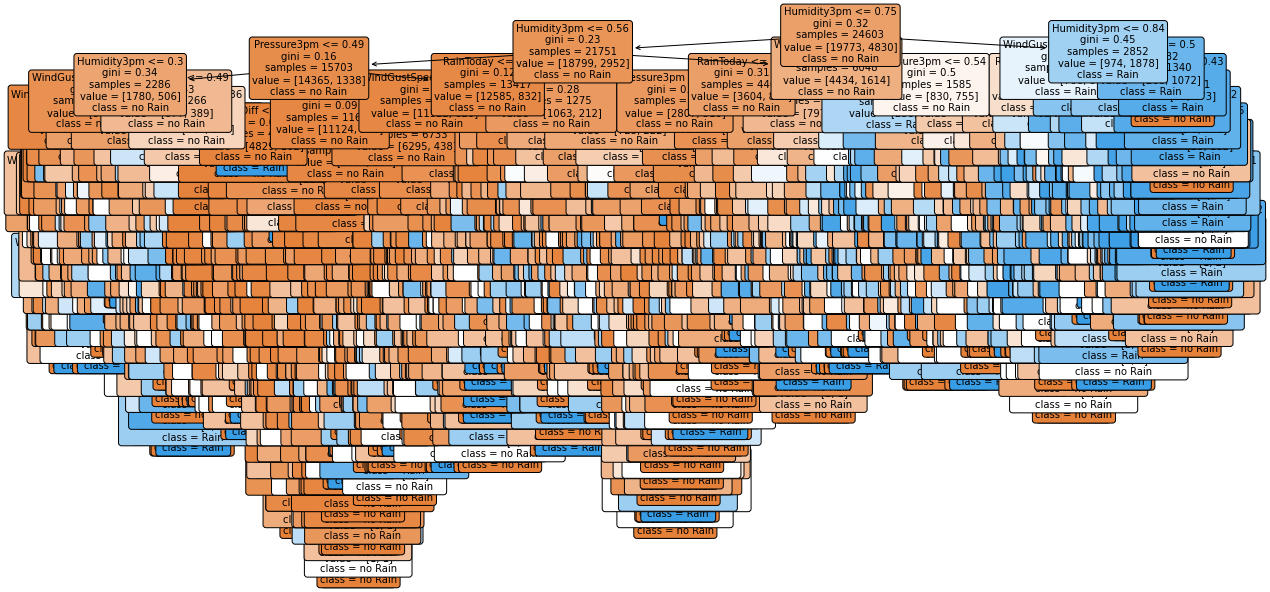
\includegraphics[width=0.31\textwidth]{Bilder/treedefault}\label{fig:treedefault}}
	\hfill
	\subfloat[\emph{max\_depth = 5}]{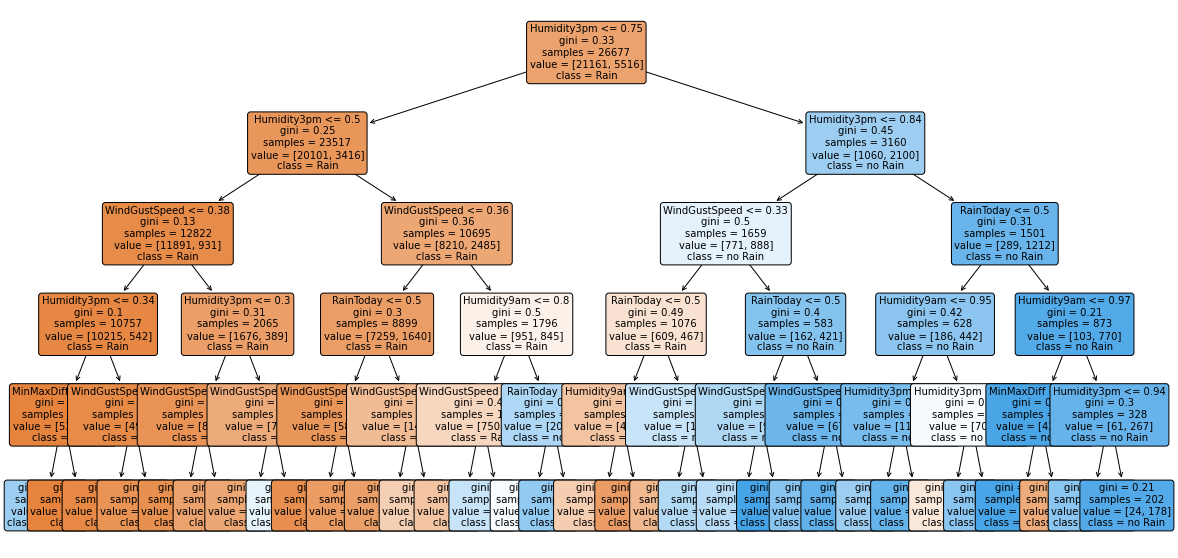
\includegraphics[width=0.30\textwidth]{Bilder/treeMaxDepth}\label{fig:treeMaxDepth}}
	\hfill
	\subfloat[\emph{min\_impurity\_decrease = 0.001}] {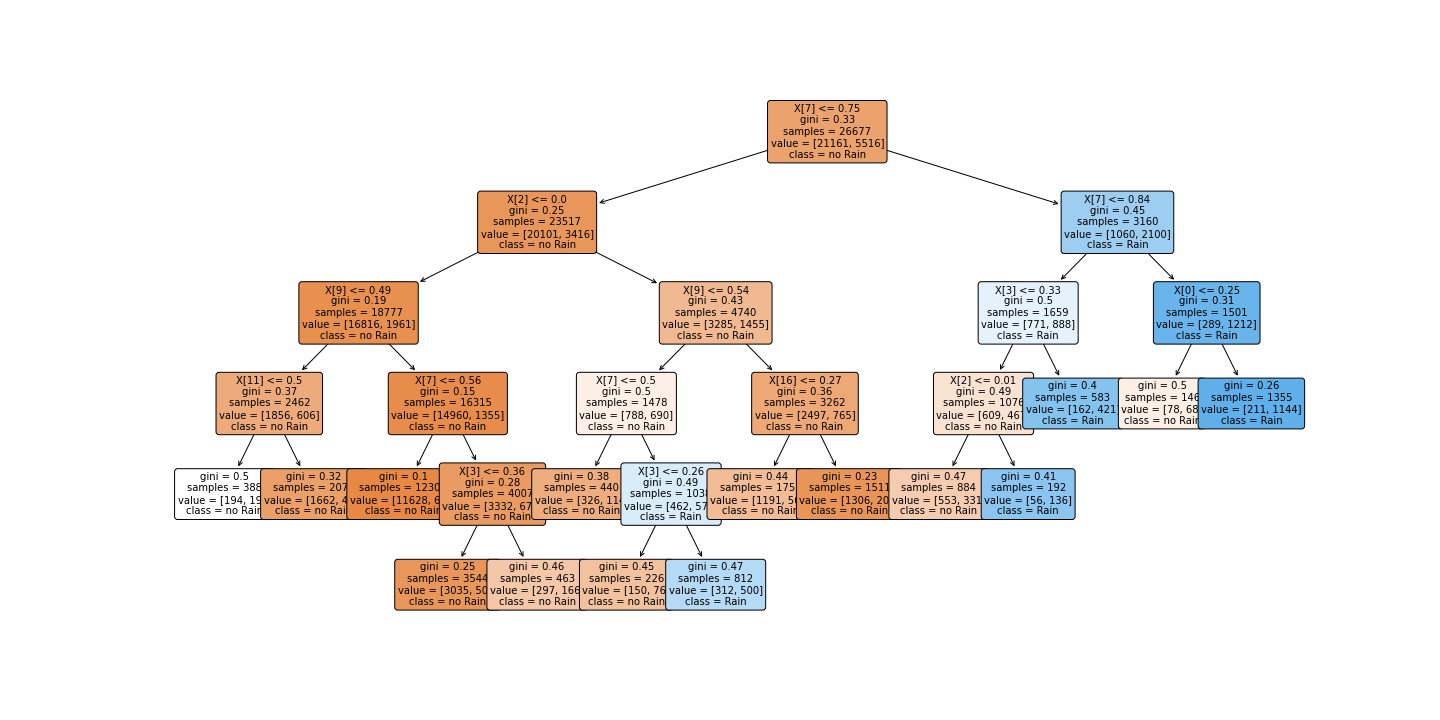
\includegraphics[width=0.30\textwidth]{Bilder/treeMinImpurityDecrease}\label{fig:treeMinImpurityDecrease}}
	\caption{Entscheidungsbäume mit Parameter-Variation}
\end{figure}

\begin{comment}
Auf den Abbildungen \ref{fig:treeMaxDepth} bis \ref{fig:treeCriterion} sind exemplarisch Entscheidungsbäume dargestellt, deren Parameter empirisch festgelegt wurden. Bei der Visualisierung liegt der Fokus auf der Struktur des Baumes und nicht darauf, dass die einzelnen Knoten identifiziert werden können.\\
\end{comment}
\begin{description}
	\item[\emph{max\_depth}]
	 definiert die maximale Tiefe des Entscheidungsbaumes. Tiefe Bäume neigen dazu, sich den Trainingsdaten überanzupassen. Flache Bäume dagegen neigen dazu, die Trainingsdaten unteranzupassen. Auf Abbildung \ref{fig:grid_search_max_depth_tree} aus Kapitel \ref{section:univariat} ist die Balance zwischen über- und unteranpassung mit variierender \emph{max\_depth} dargestellt. Die beste Klassifizierungsgenauigkeit konnte mit einer maximalen Tiefe von 5 erreicht werden. Eine exemplarische Darstellung der Struktur eines Entscheidungsbaums der Tiefe 5 ist in Abbildung \ref{fig:treeMaxDepth} dargestellt.

	\item[\emph{min\_impurity\_decrease}] 
	legt fest, zu welchem Anteil die Unschärfe reduziert werden muss, sodass eine Aufteilung eines Knotens stattfindet. Dies hat, wie in Abbildung \ref{fig:treeMinImpurityDecrease} zu sehen, auch eine direkte Auswirkung auf die Tiefe des Entscheidungsbaums. Das Ergebnis einer \emph{Grid Search} nach einer optimalen Einstellung von \emph{min\_impurity\_decrease} kann Abbildung \ref{fig:grid_search_impurity_decrease} entnommen werden.
	
	\item[\emph{criterion}]
	definiert das Kriterium, an dem die Qualität einer Aufteilung gemessen wird. Die \emph{scikit-learn}-Bibliothek unterstützt hierbei den Gini-Index, und eine Messung des Informationsgewinns mittels der Entropie. Die Wahl des Gini-Index liefert hierbei unabhängig von den andern beiden Hyperparameter-Einstellungen ein minimal besseres Ergebnis. Außerdem ist die Berechnung des Informationsgewinns mit Hilfe der Entropie durch die logarithmische Funktion aufwändiger. In \cite{gini_entropy} wird der Unterschied zwischen Informationsgewinn und Gini-Index näher untersucht.
\end{description}

Wie bereits erwähnt haben die beiden Hyperparameter \emph{max\_depth} und \emph{min\_impurity\_decrease} eine Auswirkung auf die Tiefe des Entscheidungsbaums. Das Setzen von \emph{min\_impurity\_decrease} anstelle von  \emph{max\_depth} hat den Vorteil, dass dies eine eher weiche Abbruchbedingung während des Trainings darstellt. Somit ist die Gefahr der Unteranpassung geringer. Die Wahl des Gini-Index als Entscheidungskriterium für eine Aufteilung liefert minimal bessere Ergebnisse und ist unaufwändiger zu berechnen. Ein Entscheidungsbaum mit der Einstellung \emph{min\_impurity\_decrease} = 5, sowie der Wahl des Gini-Index hat eine Klassifizierungsgenauigkeit von 84,5\% auf die Testdaten.

%TODO: Fazit und noch mal drüber lesen....

\subsubsection{Minimal Cost-Complexity-Pruning}
Eine Möglichkeit der Vermeidung des Overfittings bietet das \emph{Cost-Complexitiy Pruning} als sogenannte \emph{Post-Pruning}-Methode. Dabei wird der voll ausgebildete Baum iterativ beschnitten, indem diejenigen Teilbäume entfernt werden, die einen festgelegten penalisierten Fehlerterm minimieren.\\
\noindent \hspace*{7mm}
Das Modul \emph{DecisionTreeClassifier} bestimmt für jeden Knoten den effektiven $\alpha$-Wert. Dabei entpricht $\alpha_{eff}$ dem $\alpha$, für das gilt: $R_{\alpha}(T_{t})=R_{\alpha}(t)$. Der Knoten mit dem geringsten effektiven $\alpha$ wird vom Baum abgeschnitten. Dieses Vorgehen wird solange wiederholt, bis der geringste effektive $\alpha$-Wert größer als der gegebenen Penalisierungs-Term \emph{ccp\_alpha} ist.\\
\noindent \hspace*{7mm}
Dabei ist zu beachten, dass die Bäume stärker beschnitten werden, je höher der gegebene Penalisierungs-Term ist, da dieser eine hohe Anzahl an Knoten bestraft (siehe auch \ref{app:abb_booklet_1}).\\
\noindent \hspace*{7mm}
Das Pruning hat Auswirkungen auf die Modellgüte, indem es die Anpassung an die Trainingsdaten reguliert. Wird der Penalisierungs-Term zu hoch gesetzt, besteht die Gefahr der Unteranpassung, ein sehr niedriger Term führt zu Overfitting. In Abbildung \ref{fig:ccp_accuracyVsAlpha} ist beispielhaft für einen Entscheidungsbaum mit Default-Einstellungen die Trainings- und Testgenauigkeit (Accuracy) für verschiedene Pruning-Parameter $\alpha$ dargestellt.

\begin{figure}[h]
	\centering
	\vspace*{-0.8 cm}
	\subfloat[]{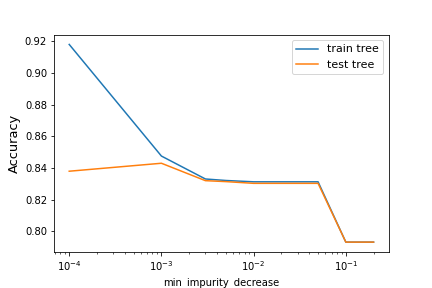
\includegraphics[width=0.53\textwidth]{Bilder/min_impurity_decrease.png}\label{fig:grid_search_impurity_decrease}}
	\hfill
	\subfloat[] {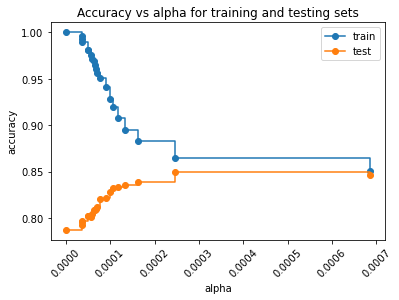
\includegraphics[width=0.45\textwidth]{Bilder/ccp_accuracyVsAlpha.png}\label{fig:ccp_accuracyVsAlpha}}
	\caption{(a): Klassifizierungsgenauigkeit eines Entscheidungsbaums abhängig des Hyperparameters \emph{min\_impurity\_decrease} (b): Trainings- und Testfehler für verschiedene $\alpha$-Werte}
\end{figure}



